%!TEX root = ../thesis.tex
%*******************************************************************************
%****************************** Second Chapter *********************************
%*******************************************************************************

\chapter{Heavy Neutral Leptons}

\ifpdf
    \graphicspath{{Chapter2/Figs/Raster/}{Chapter2/Figs/PDF/}{Chapter2/Figs/}}
\else
    \graphicspath{{Chapter2/Figs/Vector/}{Chapter2/Figs/}}
\fi

%********************************** %Opening  **************************************

Neutrino oscillation is the key evidence suggesting that neutrinos have mass, a phenomenon that cannot currently be explained by the Standard Model (SM).
This motivates an additional right-handed neutrino state that allows for the construction of the Dirac and/or Majorana mass term of neutrinos.
If the new state is very heavy, it can potentially provide a new mass generation mechanism to explain the lightness of neutrinos.
The heaviness of this new state compared to neutrinos earns it the name \textit{Heavy Neutral Lepton} (HNL).
HNLs are proposed to interact with SM gauge bosons, allowing them to be produced and decay via SM gauge interactions.
This leads to the focus of this work on the search for HNLs in the mass range of the order $\mathcal{O}$(100) MeV that are produced from the Booster Neutrino Beam and then decay into SM observables inside the Short-Baseline Near Detector at Fermilab.

The first chapter here provides an overview on the theory of HNLs and a summary of search results for their existence.  
In Section \ref{sec2Overview}, the motivation of HNLs as a minimal extension to the SM is presented.
Section \ref{sec2Production} provides the explanation for the production mechanism of HNLs from meson decays.
Following this, Section \ref{sec2Decay} covers the details of HNL decays into SM observables. 
Section \ref{sec2Previous} then summarises the existing upper limits on the mixing and mass phase space of HNLs through two different experimental methods: peak searches and decay searches.
Finally, Sec. \ref{sec2conclude} provides some brief concluding remarks.

%********************************** %First Section  **************************************
\newpage
\section{HNL Motivation}
\label{sec2Overview}

%Motivation for HNL theory: neutrino oscillation -> right handed Dirac mass term
%The first hints of neutrino oscillation emerged in 1968, when an anomaly in solar neutrino was observed by Davis et al. in the Homestake experiment \cite{Homestake}.
%Subsequent reinforcing results quickly came from Kamiokande \cite{Kamiokande}, SAGE \cite{SAGE} and GALLEX \cite{GALLEX} experiments.
%It was not until 1998 that neutrino oscillation was conclusively measured by the Super Kamiokande collaboration \cite{superK}, followed by confirmation from the SNO collaboration in 2001 \cite{SNO}. 

%However, the Standard Model (SM) is incomplete, and currently provides no mass generation for the neutrinos.
%SM neutrinos interact weakly, indicating the existence of left-handed chiral neutrino fields, but their right-handed counterparts still remain absent. 

The phenomenon of three flavour neutrino oscillation is well-established.
Active neutrinos are produced and detected as their flavour states $\nu_\mu$, $\nu_e$ and $\nu_\tau$ and the neutrino oscillation describes the neutrino flavour states changing from one flavour to another as the neutrinos propagate some distances.
Neutrino oscillation directly implies the existence of non-zero mass for at least two out of the three neutrino states.
Whilst the Standard Model (SM) of particle physics has proved extremely successful, unfortunately, it currently provides no mechanism for the mass generation of neutrinos.
The absence of a right-handed chiral partner to the left-handed chiral neutrino means that no Dirac mass term can be built via the Yukawa coupling of the Higgs to the opposite chirality fields.

%RH Mass mechanism i.e. Dirac mass term
%, enabling the construction of a Dirac mass term for neutrinos through the Yukawa coupling to the Higgs field.

This motivates an introduction of a right-handed neutrino such that the neutrino mass can be constructed using the same recipe as all other SM particles.
The Dirac mass term in the neutrino Lagrangian after spontaneous symmetry breaking is as follows \cite{Thomson}
\begin{equation}
\mathcal{L}_{D} = -m_{D} (\overline{\nu_{L}}\nu_{R} + \overline{\nu_{R}}\nu_{L}) 
\label{eq:dirac}
\end{equation}
where $m_{D} = Yv/\sqrt{2}$ is the Dirac mass, $Y$ is the Yukawa coupling, $v$ is the Higgs vacuum expectation value, and the subscript $R$ and $L$ denotes the right and left chiral state of the $\nu$ neutrino and $\overline{\nu}$ anti-neutrino field. 
While the Dirac mass term requires the existence of both left and right-handed chiral states, the Majorana mass term was proposed by Ettore Majorana in 1937 requiring only one chiral state \cite{Majorana}.
Under the condition that a particle is its own antiparticle, the charge conjugation operator $C$ can be applied to $\nu_R$ such that $\nu^{C}_{R}=C\overline{\nu_{R}}^{T}$, where the resulting $\nu_R^C$ has the correct properties to be used in place of $\nu_L$ in Eq. \ref{eq:dirac} \cite{Kim}.
The construction of the Majorana state violates the charge conservation and is forbidden for any other SM particle with an exception of neutrinos due to their neutral charges. 
In this case, the Majorana mass term in the neutrino Lagrangian is as follows \cite{Kim}
\begin{equation}
	\mathcal{L}_{M} = -\frac{1}{2}M(\overline{\nu_{R}^{C}}\nu_{R} + \overline{\nu_{R}}\nu_{R}^{C})
\end{equation}
where $M$ is the Majorana mass. 
The factor of a half is introduced to account for double counting since the term $\overline{\nu_R}$ and $\nu^C_R$ are not independent.

A right-handed neutral state provides a hypothetical neutrino mass mechanism not only via the Dirac or the Majorana mass term but also via combining both mass terms together.
A generalised Lagrangian in this case is as follows \cite{Thomson}
\begin{equation}
	\mathcal{L}_{DM} = -\frac{1}{2}[m_D\overline{\nu_{L}}\nu_{R} + m_D\overline{\nu_{R}^{C}}\nu_{L}^C + M\overline{\nu_{R}^{C}}\nu_{R}] + h.c.
\end{equation}
The Lagrangian presented here allows for the seesaw mechanism to construct the physical masses of active neutrinos assuming the Majorana mass term is much larger than the Dirac mass term, $M \gg m_D$ \cite{Thomson, nuMass}.
Under the assumption of only two neutrino states for simplification, the seesaw mechanism would give the mass of a left-handed neutrino state $m_{\nu} \approx \frac{m_D^2}{M}$ and a right-handed neutrino state $m_N$ $\approx M$, such that the heaviness of $m_N$ suppresses the physical mass of the active neutrino $m_\nu$.
Thus, a right-handed heavy neutrino state is a very attractive addition to the SM as an answer to the neutrino mass mechanism, providing an explanation for the extreme lightness of active neutrinos.

%HNL characteristisc: no charge, mass mixing, weaker-than-weak
The neutral nature of right-handed neutrinos requires all SM charges to be zero implying that they do not interact directly via the strong, electromagnetic, or weak forces.
These weaker-than-weak right-handed particles are often referred to as \textit{sterile neutrinos}.
The only direct coupling to the new sterile state is neutrino-Higgs interaction.
This leads to mixing-mediated interactions with SM gauge bosons, allowing them to be produced and decay via SM gauge interactions with a rate suppressed by the mixing \cite{SBNHNL}.
The mass range of sterile neutrinos can span over many orders of magnitudes, and the number of flavour or mass states is unconstrained.

In the mass range of the order $\mathcal{O}$(1) eV, they are known as \textit{light} sterile neutrinos and proposed to participate in oscillation with active neutrinos.
Over a short baseline distance, the addition of a single light sterile neutrino to neutrino oscillation might enhance or reduce the number of observed neutrino interactions for a given channel. 
Particularly, this model can explain the anomalies observed by the LSND and MiniBooNE experiments, where an excess of $\nu_e$ and $\overline{\nu}_e$ interactions was measured at low energy \cite{HNLWhitePaper}. 

%dedoherence stuff
In the mass range $> \mathcal{O}(10)$ eV, sterile neutrinos are now considered \textit{heavy} since their masses are significantly more massive compared to active neutrinos.
This gains them the name \textit{Heavy Neutral Leptons} (HNLs).
HNLs do not participate in oscillation with active neutrinos due to coherence loss \cite{SBNHNL}.
As a consequence of being heavier than active neutrinos, the wave packet of HNLs moves much slower compared to that of active neutrinos, and immediately undergoes propagation decoherence.
Instead, HNLs are expected to travel over some distances before decaying into SM observables.

%PMNS matrix mixing
Different theoretical models of HNLs have been developed, and a comprehensive review can be found in Ref. \cite{HNLWhitePaper}. 
In the search for HNLs presented here, the existence of HNLs will be explored in a minimal way by assuming an addition of a single HNL to the SM.  
From a generic phenomenological approach, a HNL can be added to the SM by simply extending the Pontecorvo-Maki-Nakagawa-Sakata (PMNS) matrix.
The PMNS matrix, describing the mixing of the SM neutrino flavour eigenstate $\nu_{\alpha}$ ($\alpha=e,\mu,\tau$), and the mass eigenstate $\nu_{i}$ ($i=1,2,3$), is as follows 
\begin{equation}
	U_{PMNS} =
	\begin{pmatrix}
		U_{e1} & U_{e2} & U_{e3}\\
		U_{\mu1} & U_{\mu2} & U_{\mu3}\\
		U_{\tau1} & U_{\tau2} & U_{\tau3}\\
	\end{pmatrix}
\end{equation}
The flavour eigenstate $\nu_{\alpha}$ undergoes weak interaction, whilst the mass eigenstate $\nu_{i}$ describes the neutrino propagation in space and time.
For an addition of a single right-handed neutrino with mass $m_{N}$, the PMNS matrix can be extended to describe the mass mixing between SM neutrinos and the new flavour eigenstate $N$ as follows 
\begin{equation}
	U_{PMNS}^{Extended} =
	\begin{pmatrix}
		U_{e1} & U_{e2} & U_{e3} & U_{e4}\\
		U_{\mu1} & U_{\mu2} & U_{\mu3} & U_{\mu4}\\
		U_{\tau1} & U_{\tau2} & U_{\tau3} & U_{\tau4}\\
		U_{N1} & U_{N2} & U_{N3} & U_{N4}\\
	\end{pmatrix}
\end{equation}
where the index 4 is reserved as a new mass eigenstate.
Then, the flavour eigenstate  $\nu_{\alpha}$ of SM neutrinos can be written as the linear combination of the mass eigenstate $\nu_{i}$ and the HNL flavour eigenstate $N$ as follows 
\begin{equation}
	\nu_{\alpha}=\sum_i U_{\alpha i}\nu_{i} + U_{\alpha 4}N
\end{equation}
where the mixing $U_{\alpha i }$ ($\alpha=e,\mu,\tau$ and $i=1,2,3$) are elements of the SM PMNS matrix, and the mixing $U_{\alpha 4}$ are the extension.
For simplicity, this work only considers a HNL coupling to only one flavour at a time, such that at most one of the three mixing $U_{e4}$, $U_{\mu4}$ and $U_{\tau4}$ is non-zero.

%Available mass range 
%The HNL mass range of interest must be able to be produced from the Booster Neutrino Beam (BNB) and directly detected by the Short-Baseline Near Detector (SBND), which limits the probable mass range to $\mathcal{O}$(100 MeV).
%At this mass range over a baseline distance of 110 m, oscillation with active neutrinos results in coherence loss \cite{SBNHNL}.
%Instead, HNLs are expected to travel over a long distance before decaying into SM observables via mass mixing.

%This thesis: simple phenomenological model
%Example model: minininal neutrino extension of the SM
%The HNLs have been predicted by many different models, where a comprehensive overview has been discussed here \cite{}.
%A particular model requires a minimum extension to the SM has been presented, \textit{Neutrino Minimal Extension of the SM} ($\nu$MSM)\cite{}.
%The model introduces three generations of HNLs.
%The two heavier ones N$_{1,2}$ in the mass range of $\mathcal{O}$(10 GeV) and $\mathcal{O}$(100 MeV) can generate the mass of active neutrinos via the See-saw mechanism, whilst the third and lightest N$_{3}$ with keV mass can be a viable dark matter candidate.
%$\nu$MSM also accounts for the currently observed matter-antimatter asymmetry for having the heavy HNLs oscillating in a charge and parity violating manner during the early universe, dubbed leptogenesis via neutrino oscillations. 
 
\section{HNL Production}
\label{sec2Production}
%Decay mechanism: replace SM with a HNL -> mixing
In any SM neutrino production processes, HNLs can be produced in place of neutrinos with a rate suppressed by the mixing $|U_{\alpha4}|^{2}$, if kinematically allowed. 
Fig. \ref{fig:kaonnu} illustrates the two-body decay of a charged kaon $K^+$ producing a muon neutrino $\nu_{\mu}$ and Fig. \ref{fig:kaonhnl} illustrates the substitution of the $\nu_{\mu}$ with a HNL $N$ having $L = +1$ mediated by the mixing $|U_{\alpha4}|^{2}$. 
This implies that HNLs can be probed from the Booster Neutrino Beam (BNB), which is an abundance source of mesons and will be further detailed in Sec. \ref{sec4BNB}.
Since the BNB is primarily made up of positively charged mesons, the following section will focus on the parent meson $K^+$ and $\pi^+$.  

\begin{figure}[ht!]
%\hfill
\begin{subfigure}[h]{0.4\linewidth}
\centering    
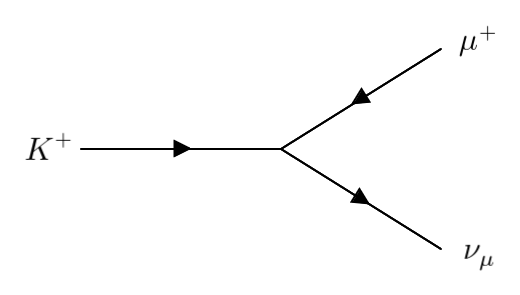
\includegraphics[width=\linewidth]{K_to_nu}
\caption{}
\label{fig:kaonnu}
\end{subfigure}
\hfill
\begin{subfigure}[h]{0.4\linewidth}
\centering    
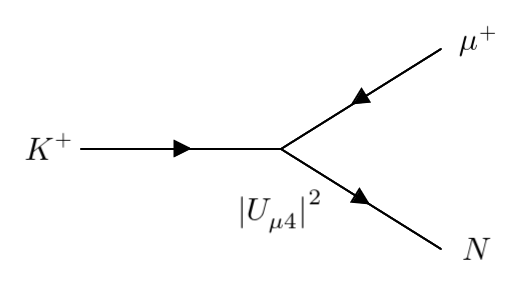
\includegraphics[width=\linewidth]{K_to_HNL}
\caption{}
\label{fig:kaonhnl}
\end{subfigure}%
%\hfill
\caption[kaonDiagram]{
	Feynman diagrams of (a) $K^+ \rightarrow \mu^+ \nu_{\mu}$ and (b) $K^+ \rightarrow \mu^+ N$.% \cite{DavidePhD}.
}
\end{figure}

In general, the branching ratio $Br(m^+\rightarrow l^{+}_{\alpha}N)$ of a two-body decay of a charged meson $m^+$ into a lepton $l^{+}_{\alpha}$ ($\alpha=e,\mu,\tau$) and a HNL $N$ can be expressed in terms of the analogous branching ratio into a SM neutrino as follows \cite{HNLKelly}
\begin{equation}
	\label{eq:kaon_decay_hnl}
	Br(m^+\rightarrow l^{+}_{\alpha}N) = Br(m^+\rightarrow l^{+}_{\alpha}\nu_{\alpha})\left(\frac{|U_{\alpha 4}|^{2}}{1 - |U_{\alpha 4}|^{2}}\right)\rho_{N}\left(\frac{m^{2}_{l_{\alpha}}}{m^{2}_{m^+}}, \frac{m^{2}_{N}}{m^{2}_{m^+}} \right) 
\end{equation}
where $Br(m^+\rightarrow l^{+}_{\alpha}\nu_{\alpha})$ is the branching ratio of the charged lepton $m^+$ decaying into a lepton $l^+_{\alpha}$ and a SM neutrino $\nu_{\alpha}$, $m_{m^+}$ is the mass of the charged meson, $m_{l_{\alpha}}$ is the mass of the daughter lepton and $m_{N}$ is the mass of the daughter HNL.
The kinematic factor $\rho_{N}$ accounts for the available phase space of the daughter HNL in the decay and has the complete expansion as follows \cite{HNLKelly}

\begin{equation}
	\rho_{N}(x,y) = \frac{(x+y-(x-y)^{2})\sqrt{1+x^{2}+y^{2}-2(x+y+xy)}}{x(1-x)^{2}}
\label{eq:KinematicsFactor}
\end{equation}
where $x = m^{2}_{l_{\alpha}}/m^{2}_{m^+}$ and $y=m^{2}_{N}/m^{2}_{m^+}$.

Fig. \ref{fig:KinematicsFactor} depicts the kinematic factor $\rho_N$ of the HNL production compared to the analogous SM neutrino production as a function of the HNL mass.
Four HNL production channels that are probable at the BNB are shown: (1) $K^+ \rightarrow Ne^+$ in the dashed red line, (2) $K^+ \rightarrow N\mu^+$ in the solid pink line, (3) $\pi^+ \rightarrow Ne^+$ in the dashed dark blue line and (4) $\pi^+ \rightarrow N\mu^+$ in the solid light blue line.  
Production channels associated with the $\tau$-flavour mixing are not shown since they are kinematically forbidden at the BNB.
The kinematic factor for each illustrated channel is constrained by the available mass after the two-body decay of the parent meson, and the upper limit of the HNL mass is $m_{N} = m_{m^+} - m_{l_{\alpha}}$ ($\alpha=e,\mu$), as shown by the vertical grey lines.
Here it can be seen that the HNL production from $\pi^+$ decays limits the HNL mass to $< 140$ MeV while the HNL production from $K^+$ decays allows for the HNL mass up to 495 MeV. 
Thus, the search for HNLs presented here focuses on the HNL production channel from $K^+$ to probe mass as high as 495 MeV.

%Given the smaller masses of both a charged pion ($m_{\pi} = 140 $ MeV) and a charged kaon ($m_{K} = 494 $ MeV) compared to a tau ($m_{\tau}=1777 $ MeV), taus cannot be produced from meson decays in the BNB.
%Consequently, only electrons and muons are produced, limiting the flavours in the mixing $|U_{\alpha4}|^{2}$ to $\alpha = e, \mu$.

%Helicity Unsuppression i.e. K ->Ne and K->Nmu

%Enahancement factor??

Furthermore, the magnitude of the kinematic factor of the HNL production shown in Fig. \ref{fig:KinematicsFactor} is larger than 1 as compared to the analogous SM production.
This is because of the helicity suppression observed in mesons decaying into a SM neutrino having an opposite effect for mesons decaying into a HNL \cite{HNLKelly}.
Instead, it is helicity \textit{enhancement} due to HNLs being massive.
For the HNL production channel interested in this work, a significant enhancement is evident for the production rate of $K^+\rightarrow e^+ N$ being increased by a factor of $10^{5}$.
On the other hand, the kinematic factor of $K^+ \rightarrow \mu^+ N$ unfortunately only peaks at 4, implying a negligible enhancement on the production rate. 

%The kinematic factor $\rho_{N}$ from Eq. \ref{eq:KinematicsFactor}, which also accounts for this enhancement, is plotted against the mass of HNLs in Fig. \ref{fig:KinematicsFactor}.

\begin{figure}[t] 
\centering    
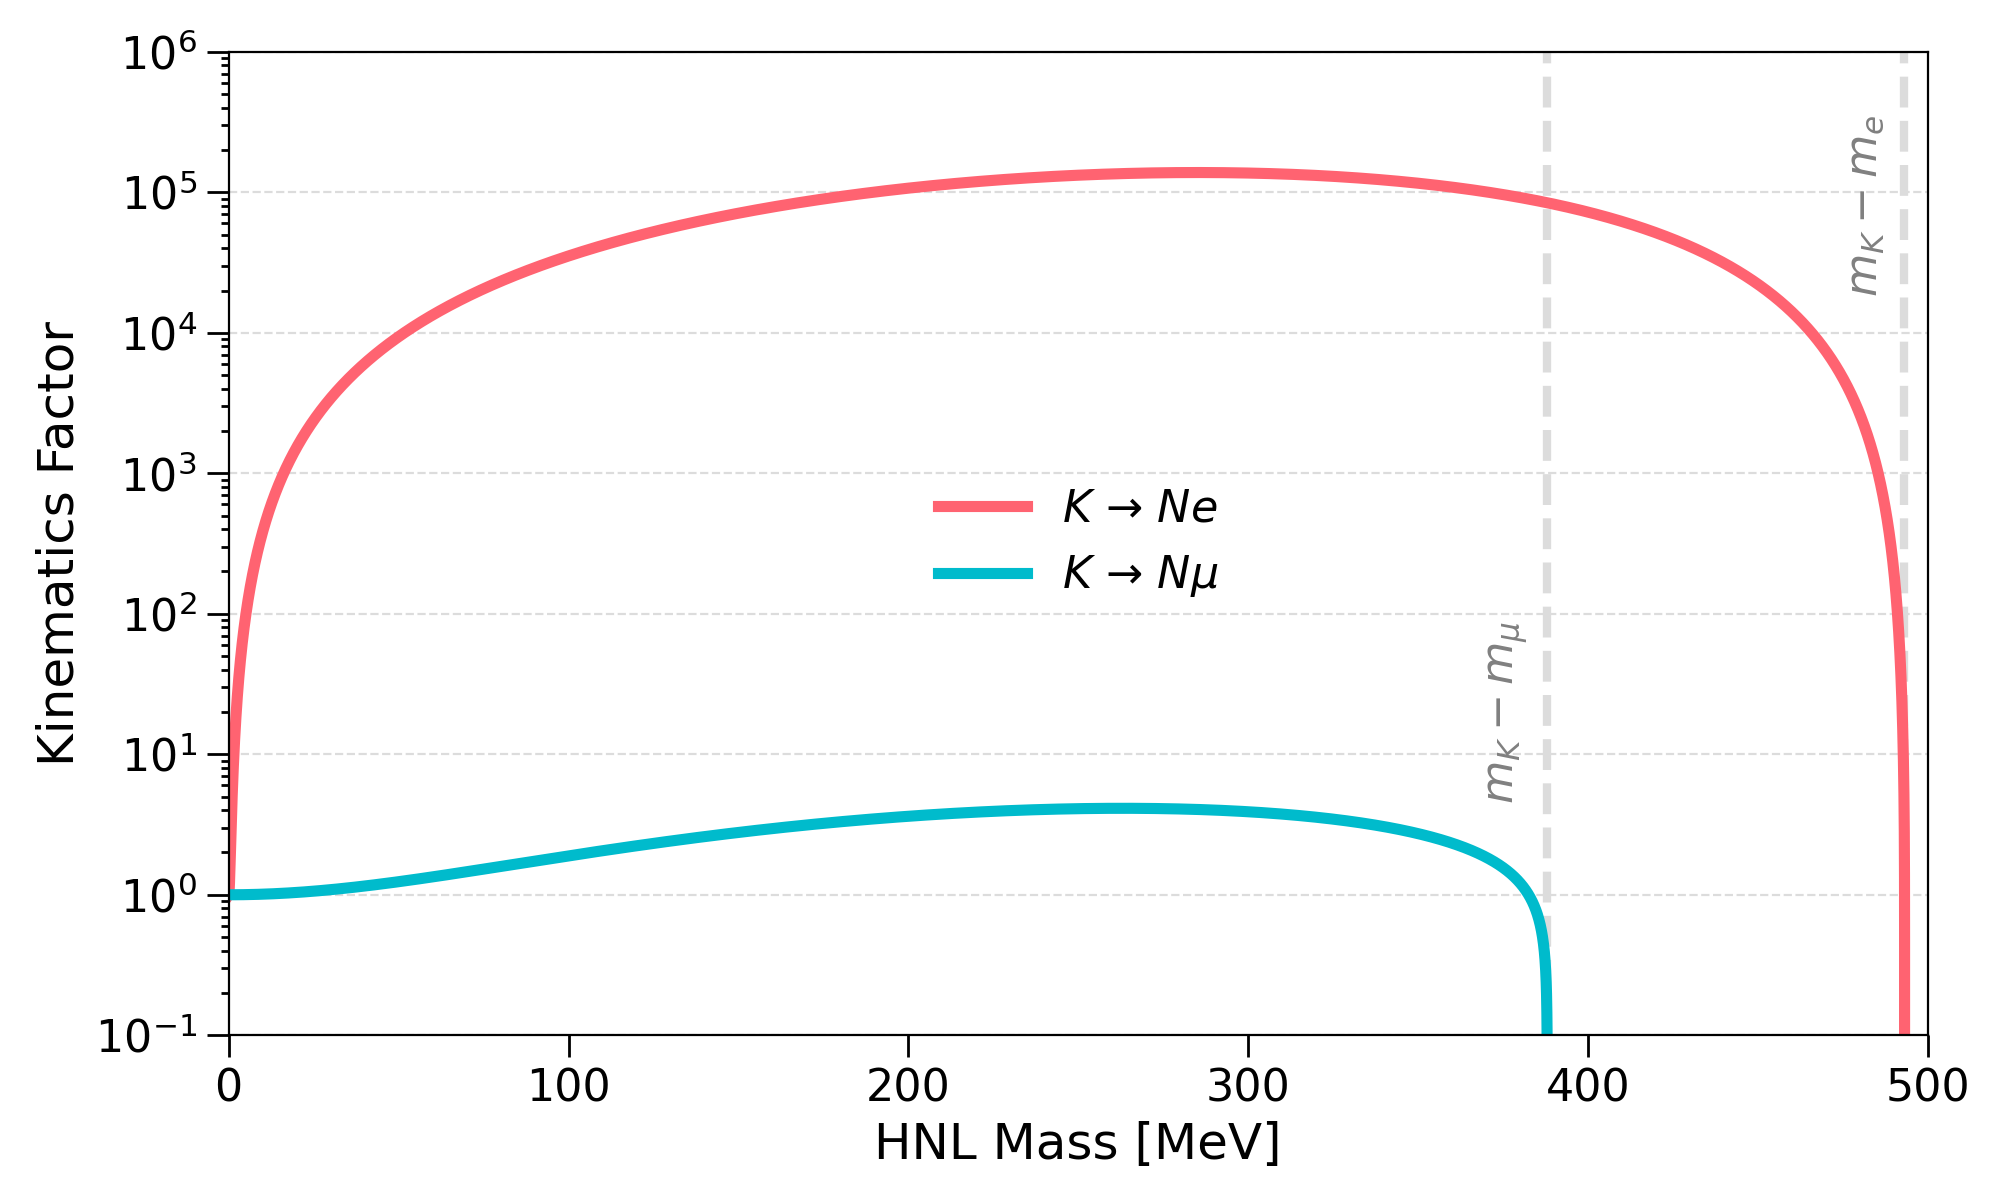
\includegraphics[width=1.0\textwidth]{kinematics_factor}
\caption[KinematicsFactor]{
Plot showing the kinematic factor of the HNL production from meson decays as compared to the analogous SM neutrino production.
}
\label{fig:KinematicsFactor}
\end{figure}

\section{HNL Decay}
\label{sec2Decay}

%HNLs are unstable particles and therefore decay in flight with a lifetime proportional to the mixing $|U_{\alpha4}|^{2}$ $(\alpha=e,\mu,\tau)$, 
%Since $|U_{\alpha4}|^{2}$ is the same coupling responsible for the HNL production, the observed event rate at the detector scales with $|U_{\alpha4}|^{4}$.

%DIF with coupling
For HNLs to be detected, they are hypothesised to be able to decay into SM observables \cite{HNLKelly}.
The proposed lifetime of HNLs should be sufficient so that a HNL produced from the BNB must survive long enough to reach the detector and then decay in flight.
At the mass range $< 495$ MeV, the kinematically-allowed decay channels of a HNL are as follows \cite{SBNHNL}

%Possible decay channel
\begin{equation}
\begin{split}
\label{eq:decay_channel}
	N\rightarrow e^{-}\pi^{+},\qquad 
	N\rightarrow \mu^{-}\pi^{+},\qquad
	N\rightarrow \nu \pi^{0},\qquad 
	N\rightarrow \nu \gamma,\qquad \\ 
	N\rightarrow \nu e^{-} e^{+},\qquad 
	N\rightarrow \nu \mu^{-} \mu^{+},\qquad 
	N\rightarrow \nu \mu^{-}e^{+},\qquad
	N\rightarrow \nu \nu \nu.   
\end{split}
\end{equation}
These decay channels here conserve the lepton number under the assumption that HNLs are Dirac particles with $L=+1$.
If HNLs are Majorana particles, such that the lepton number conservation is violated, then the charge conjugates for these decays that would be forbidden in the Dirac case are now allowed.

%Overall description of each BR channel

Fig. \ref{fig:branchingRatio} depicts branching ratios of decay channels shown in Eq. \ref{eq:decay_channel}, as a function of the HNL mass.
Solid lines are branching ratios via the $\mu$-flavour mixing ($[U_{e4}:U_{\mu4}:U_{\tau4}]=[0:1:0]$) and dashed lines are branching ratios via the $e$-flavour mixing ($[U_{e4}:U_{\mu4}:U_{\tau4}]=[1:0:0]$).
The branching ratios were plotted referencing decay widths from Ref. \cite {HNLBin, SBNHNL, HNLZarko}.
Decay widths of HNLs have been derived independently across various literature sources and an overview of discrepancies is summarised in Ref. \cite{HNLZarko}. 
The sources used here have been found to be in good agreement with each other.

For $m_{N} < 135$ MeV, the dominant branching ratio occurs in the channel $N\rightarrow \nu\nu\nu$ as shown by the light green lines.
However, this channel is almost unobservable since the detection of SM neutrinos relies on the already-small cross section of neutrino scattering with the detector material.
The other two channels in this mass range are $N\rightarrow \nu e^{-}e^{+}$ and $N\rightarrow \nu \gamma$, as shown by the light pink and grey lines.
The channel $N\rightarrow \nu \gamma$ is highly suppressed compared to the channel $N\rightarrow \nu e^{-}e^{+}$, and thus, the final state of $e^-e^+$ pair provides the best sensitivity within this mass range.

For $m_{N} > 135$ MeV, a HNL has sufficient mass to decay into either a neutral pion ($m_{\pi^{0}}=135$ MeV) or a charged pion ($m_{\pi^{+}}=140$ MeV). 
For the $e$-flavour mixing, the channel $N\rightarrow e^{-}\pi^{+}$ dominates over the channel $N\rightarrow \nu \pi^{0}$ across the mass range from 135 to 495 MeV, as shown by the dashed dark blue and dashed pink line respectively.
In the case of the $\mu$-flavour mixing, the leading channel within the mass range of $135 < m_{N} < 245 $ MeV is $N\rightarrow \nu \pi^{0}$ as shown by the solid pink line.
Beyond $m_{N} > 245$ MeV, equivalent to the mass of a muon and a charged pion, the dominant decay channel begins to shift to the channel $N\rightarrow \mu^{-}\pi^{+}$ as shown by the solid blue light. 
Finally, both channels $N\rightarrow \nu \mu^{-}e^{+}$ and $N\rightarrow \nu \mu^{-}\mu^{+}$ are not competitive compared to any other channels at the same mass value.  

\begin{figure}[ht!] 
\centering    
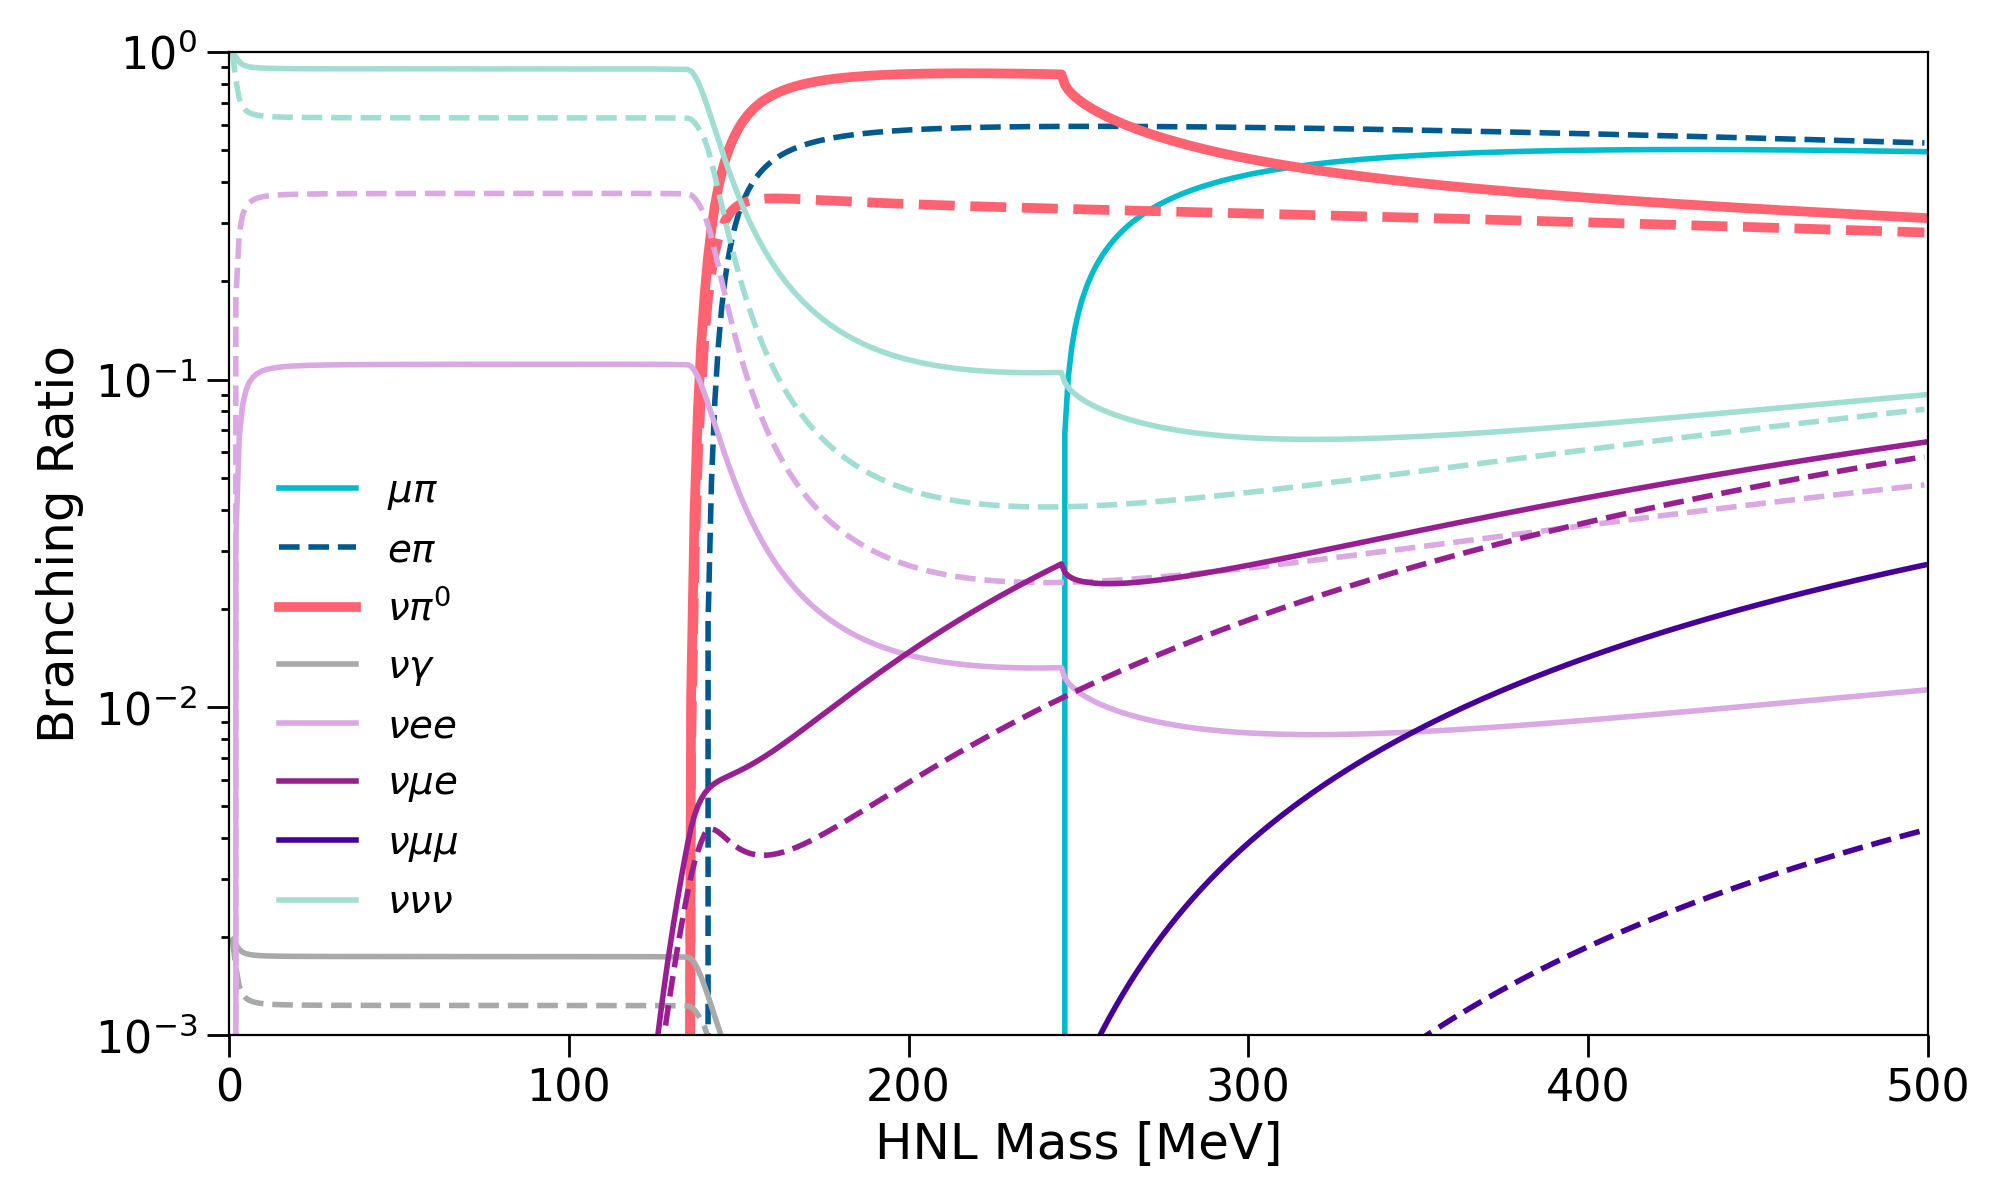
\includegraphics[width=1.0\textwidth]{branching_ratio}
\caption[branchingRatio]
{
Plot showing the branching ratio of probable decay channels of a HNL produced from the BNB.
}
\label{fig:branchingRatio}
\end{figure}

%This prompts a search focus on non-zero $|U_{\mu4}|^{2}$, assuming $|U_{e4}|^{2} = |U_{\tau4}|^{2} = 0$.  
%In this mass range, the primary mode of HNL production comes from  the decay of charged kaon, due to the kinematic constrains (See Sec. \ref{sec2Production}). 

Based on the assessment above it was decided in this work to focus on searching for HNLs through the decay channel $N\rightarrow\nu \pi^{0}$, which will be covered in Chapter \ref{ChapterSelect} and \ref{ChapterResult}.  
This is the leading channel of the $\mu$-flavour mixing within the mass range of $ 135 < m_{N} < 245 $ MeV.
Sensitivity in the same mass range of the $e$-flavour mixing has been extensively explored by many experiments as summarised by Ref. \cite{HNLWhitePaper}.
The decay width for the $N\rightarrow\nu \pi^{0}$ channel as taken from Ref. \cite{HNLZarko} is as follows
\begin{equation}
	\Gamma(N\rightarrow \nu \pi^{0}) = \frac{G_{F}^{2}m_{N}^{3}}{32\pi}f^{2}_{\pi}|U_{\mu4}|^{2}\left(1-\left(\frac{m_{\pi^{0}}}{m_{N}}\right)^{2}\right)^{2}
\label{eq:pi0}
\end{equation}
where $G_{F}$ is the Fermi constant, $f_{\pi}$ is the pion decay constant and $m_{\pi^{0}}$ is the mass of a neutral pion.
It is noted that the equivalent equations from Ref. \cite{SBNHNL, HNLBin} contain an additional factor of 2 in the denominator.
Eq. \ref{eq:pi0} was chosen from Ref. \cite{HNLZarko} since the source is more recently dated. 

%Decay signature in TPC
Fig. \ref{fig:HNLdecaydiagram} shows the diagram of the HNL decaying into the final state $\nu\pi^0$.
The SM neutrino is expected to leave no detectable signatures due to their very small scattering cross sections.
Meanwhile, the neutral pion is very short-lived with a mean lifetime of $8.52\pm0.18 \times 10^{-17}$ s and decays into two photons $98.823 \pm 0.034 \%$ of the time \cite{PDG}. 
Fig. \ref{fig:pi0decaydiagram} shows the Feynman diagram for the described decay.
The photon pair results into clear a signature inside a Liquid Argon Time Projection Chamber (LArTPC): two electromagnetic showers without any associated hadronic activities at the decay vertex.
This signal topology will face very challenging background separation from some SM neutrino channels also containing a $\pi^0$ in the final state.
As described in more detail in Chapter \ref{ChapterSelect}, differences in the final state kinematics from the HNL signal to the SM neutrino background enable an effective separation.

%this interaction constitutes the main background in
%Neutral current neutrino interactions that result in a neutral pion also share the same final state particles and thus, constituting the main background for this search.

%Nonetheless, . 

\begin{figure}[htbp!]
%\hfill
\begin{subfigure}[h]{0.49\linewidth}
\centering    
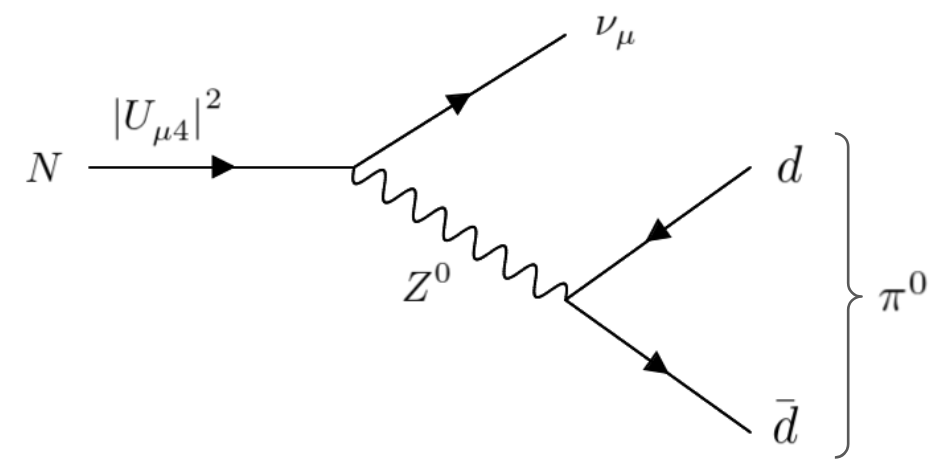
\includegraphics[width=\linewidth]{N_to_pi0_edit}
\caption{}
\label{fig:HNLdecaydiagram}
\end{subfigure}
\hfill
\begin{subfigure}[h]{0.49\linewidth}
\centering    
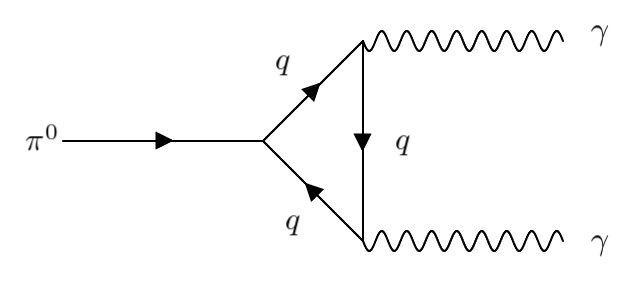
\includegraphics[width=\linewidth]{pi0_to_gam}
\caption{}
\label{fig:pi0decaydiagram}
\end{subfigure}%
%\hfill
\caption[decayDiagram]{
Feynman diagrams of (a) $N \rightarrow \nu \pi^0$ and (b) $\pi^0 \rightarrow \gamma\gamma$.
}
\end{figure}

%Dirac or Majorana Nature
%Dirac HNLs conserves the lepton number, while Majorana HNLs violates the conservation and allows for forbidden decay channels    
%Majorana HNLs violate the conservation of lepton numbers, whereas Dirac HNLs preserve it.
%Consequently, the expected event rate of Majorana HNLs is double that of Dirac HNLs.

%Moreover, the polarisation of decay products differs between Majorana and Dirac HNLs for a neutral current process such as $\nu\pi^{0}$.

As discussed in Sec. \ref{sec2Production}, HNLs can be either Dirac or Majorana particles in nature.
The difference between Dirac and Majorana HNLs is not only the lepton number conservation but also the polarisation of the decay products.
For the neutral current final state $\nu\pi^0$, Majorana HNLs decay isotropically, whereas in the case of Dirac HNLs, the angular distribution of the daughter particles is no longer isotropic.
The helicity of the daughter neutrino determines the direction of the daughter neutral pion and the angular distributions of the two charge conjugate final states, $\nu\pi^{0}$ and $\overline{\nu}\pi^{0}$, add up to an isotropic distribution  \cite{HNLSilvia}.
As the neutrino is undetectable, the observed angular distribution of the neutral pion is expected to be insufficient to determine the Dirac or Majorana nature of HNLs.
For simplicity in this search for HNLs via the channel $\nu\pi^0$, it is therefore assumed that HNLs are Majorana particles.

\section{Previous Experimental Searches For HNLs}
\label{sec2Previous}

%Number of fermion families = Z boson decay for LH neutrinos, RH neutrinos is not constrained

%Overview of different types of searches
Searches for HNLs have been conducted by various experiments over the decades across a wide range of mass.
Oscillation experiments and precise $\beta$ decay experiments have probed HNLs in the mass range between eV and keV, neutrino beam dump experiments have targeted the MeV-scale HNLs and the collider experiments have primarily explored HNLs with masses in the GeV-scale and above.
To date, no evidence of HNL existence has been found, and thus, experiments have set upper limits on the mixing $|U_{\alpha4}|^{2}$ $(\alpha=e,\mu,\tau)$.
Commonly, the contour on the experiment sensitivity is expressed in terms of the mixing $|U_{\alpha4}|^{2}$ as a function of the HNL mass.

Here, current experimental limits on HNLs around $\mathcal{O}$ (100 MeV) are presented, focusing specifically on the mass range of $ 0 < m_{N} < 265 $ MeV, which is relevant to the final states $\nu\pi^{0}$.
In this mass range, two key experimental methods are used, so-called peak searches and decay searches.
Peak searches probe only the production rate of HNLs, whereas decay searches probe both production and decay rates.
Fig. \ref{fig:Sensitivity} summarises the presented upper limits at 90\% confidence level (C.L.) from both experimental methods, with details on individual limit to be discussed in Sec. \ref{sec:peaksearch} and \ref{sec:decaysearch}.

\subsection{Peak Searches}
\label{sec:peaksearch}

Peak search experiments measure the energy spectrum  resulting from the decay of meson decay that would produce a HNL. 
Typically, the two-body leptonic decay of a meson is modelled as $m\rightarrow l + Missing$, where $m$ is the parent meson, a pion or a kaon, and $l$ is the daughter particle, a pion or a lepton \cite{OwenPhD}.
The \textit{missing} decay products are attributed to either HNLs or SM neutrinos.
HNLs are expected to exit the detector before decaying, whereas SM neutrinos escape the detector before interacting, serving as the primary background for this search.
Since the momenta of $m$ and $l$ are precisely measured, the missing invariant mass can therefore be derived as $m^{2}_{miss} = (P_{m} - P_{l})^{2}$, where $P_{m}$ and $P_{l}$ are the 4-momenta of the parent and daughter particle.
Given the near-zero mass of SM neutrinos, the mass of the daughter HNL can be treated as $m_{N} = m_{miss}$.
Consequently, an excess over the background at $m_{miss}$ potentially indicates the existence of HNLs.

To infer the upper limits on the mixing parameter, the flavour $\alpha$ ($\alpha =\mu,e$) of the daughter lepton determines the flavour of the mixing $|U_{\alpha4}|^2$, and the amplitude of the decay spectrum at $m_{miss}$ determines the upper limit.
Limits placed by the peak searches are insensitive to the Dirac or Majorana nature of HNLs as it does not impact the kinematics of the meson decay.
For the mixing $|U_{\mu4}|^{2}$, the most competitive limits have been established by the following experiments on the pion and kaon decay spectrum, and are plotted in Fig. \ref{fig:Sensitivity} as dashed and dotted lines.

\subsubsection{Pion Decay Spectrum Peak Searches}

\begin{coloritemize}
\item \textbf{SIN} (Swiss Institute for Nuclear Research) performed a peak search using stopped positive pions decay via the channel $\pi^{+} \rightarrow \mu^{+} + Missing$, with a scintillator in 1981 and a germanium detector in 1987.
The pion enabled probing HNLs within the low mass range of $\mathcal{O}$(10 MeV).
Upper limits of $|U_{\mu4}|^{2}$ were placed in the mass range 1--20 MeV at $10^{-4}$ \cite{SIN1, SIN2, SIN3}.

\item The \textbf{PIENU} collaboration at TRIUMF also searched for HNLs using stopped pions.
The most recent result in 2019 set the most stringent limits on $|U_{\mu4}|^{2}$ at $10^{-5}$ in the mass range of 15--34 MeV \cite{PIENU}, extending beyond the result reported by SIN.

\end{coloritemize}

\subsubsection{Kaon Decay Spectrum Peak Searches}

\begin{coloritemize}
\item The \textbf{KEK} collaboration conducted an experiment known as E89, which aimed to search for HNLs using the muon range spectrum resulting from stopped kaon decays during 1981--1982. 
Following this, experiment E104 in 1983 was carried out with an improved momentum resolution and background suppression.
The kaons were produced using a 0.5 GeV proton beam, and $3 \times 10^{6}$ muons from kaon decays were analysed using magnetic spectrograph.
The E89 experiment result set limits on $|U_{\mu4}|^{2}$ between 10$^{-4}$--10$^{-6}$ within the mass range of 70--300 MeV.
Additionally, the combined results from the E89 and E104 experiments extended the sensitivity towards the lower mass range between 45--300 MeV, although these findings are unpublished at the time of writing \cite{KEK1, KEK2, KEK3}.

\item The \textbf{E949} collaboration at Brookhaven National Laboratory performed a kaon decay experiment using 21.5 GeV protons in 2002.
The analysis on the decays of $2 \times 10^{21}$ stopped kaons set limits on $|U_{\mu4}|^{2}$ at 10$^{-7}$--10$^{-9}$ within the mass range of 175--300 MeV \cite{E949}.

\item The \textbf{NA62} collaboration, a kaon decay experiment at the CERN super proton synchrotron, analysed $10^{8}$ stopped kaons from 400 GeV protons extracted from the synchrotron.
The first results from a data set in 2015 set upper limits on $|U_{\mu4}|^{2}$ at 10$^{-7}$--10$^{-6}$ for the HNL mass between 250--373 MeV.
Updated results using a larger dataset collected in 2016--2018 significantly improved the limits by an order of magnitude to 10$^{-8}$--10$^{-7}$, and extended the mass range to 200--384 MeV \cite{NA62A, NA62B}.
\end{coloritemize}

\subsection{Decay Searches}
\label{sec:decaysearch}

Decay searches look for decay products from HNLs.
HNLs are hypothesised to be produced outside of the detector and then decay in flight into SM observables inside the detector.
Different combinations of HNL production and decay channels yield different observed event rates of the decay products.
The flavour of the HNL production and decay channel both determine the flavour of the mixing $|U_{\alpha4}|^2$ and the observed event rate determines the upper limit on the mixing.  

Historically, decay searches have been performed in beam-dump experiments, which were designed explicitly to suppress SM background and thereby enabling the search for rare decay processes.
Recently, modern neutrino oscillation experiments have emerged as competitive beam-dump experiments alongside their neutrino physics programme.
This is due to the resolution enhancement in their detection technologies that enables excellent SM background rejection, of which the Short-Baseline Near Detector is a prime example to be further detailed in this work. 
For the mixing $|U_{\mu4}|^{2}$ within the mass range of 0--245 MeV, the most competitive limits have been set by the following experiments using neutrino beams, and are plotted in Fig. \ref{fig:Sensitivity} as solid lines.

\begin{coloritemize}
%\item The \textbf{Super-Kamiokande} (SuperK) collaboration is the only decay search presented here that searched for HNLs from a non-beam source.
%Their dataset comprised of multi-GeV atmospheric neutrinos.
%In this case, HNLs were assumed to be produced from kaon and pion decays in atmospheric showers and consequently decay inside the SuperK detector.
%The result set a limit on $|U_{\mu4}|^{2}$ at $10^{-4}$--$10^{-7}$ within the HNL mass ranging from 70 to 386 MeV \cite{superk}.


\item The CERN \textbf{PS191} experiment in 1984 utilised an exposure of 19.2 GeV protons on a beryllium target, generating $10^{19}$ protons on target (POT).
The detector was positioned at 128 m from the target at an off-axis angle of $2.3^{\circ}$ to the beam.
The detector volume was filled with helium, which was a sparse medium to reduce background rates arising from SM neutrino interactions.
The large volume of 216 m$^3$ provided a high rate of HNL signals. 
Limits on $|U_{\mu4}|^{2}$ within the mass range of 120--350 MeV were placed at the level of 10$^{-5}$--10$^{-9}$ \cite{PS191A, PS191B}.
A re-evaluation in 2022 found the limits to be lower than the original published results \cite{PS191C}.
	
%\item The \textbf{T2K} collaboration recently searched for HNLs using the near detector ND280, located 280 m from the beam target at an off-axis angle of $2.04^{\circ}$.
%The analysis was performed on the data collected from 2010-2017, with a beam intensity of 30 GeV proton on graphite target and an exposure of $\approx 2 \times 10^{21}$ POT.
%The search was limited to the three argon gas TPC volumes, which minimised the neutrino background rate due to the low gas density.
%The results constrained the limits of $|U_{\mu4}|^{2}$ in the range of 10$^{-8}$--10$^{-9}$ for the HNL mass between 250--380 MeV \cite{T2KHNL}.
%The T2K collaboration has also presented results on $|U_{\mu4}|$ in the case where $|U_{e4}|$ and $|U_{\tau4}|$ are assumed to be non-zero and marginalised using results from other channels.

\item The \textbf{NuTeV} collaboration at Fermilab conducted HNLs searches in 1996 using a high energy neutrino beam produced by protons accelerated from the Tevatron ring.
The dataset comprised an exposure of $3 \times 10^{18}$ POT with an energy of 800 GeV.
HNLs were produced from the $D$ mesons resulting from proton collisions with the target.
This enabled an exploration of the HNL mass up to 2000 MeV, surpassing any other beam-dump experiments described here.
The experiment established limits on $|U_{\mu4}|^{2}$ at the level of 10$^{-6}$--10$^{-7}$ within the mass range of 225--2000 MeV \cite{NuTeV}.

\item The \textbf{T2K} collaboration searched for HNLs using their near detector ND280 located off-axis to the beam target at an angle of $2.04^\circ$.
Only events occurring in the three gaseous TPC volumes were selected to minimise background from SM neutrinos.
A kinematic selection was performed on a dataset of $2\times10^{21}$ POT and no signals were observed.
The result constrained the mixing $|U_{\mu4}|^2$ at the level of $10^{-8}$--$10^{-9}$ in the mass range of $250$--$380$ MeV. 
The limit plotted in Fig. \ref{fig:Sensitivity} is a single-channel limit of $K^\pm \rightarrow N\mu^\pm$ and $N \rightarrow \mu^\pm\pi^\pm$.
A more stringent limit on $|U_{\mu4}|^2$ was also presented assuming the mixing $|U_{e4}|^2$ and $|U_{\tau4}|^2$ are non-zero.
This allows for a marginalised limit on $|U_{\mu4}|^2$ derived from other mixing results, which is not directly comparable here \cite{t2k}.

\begin{figure}[t!] 
\centering    
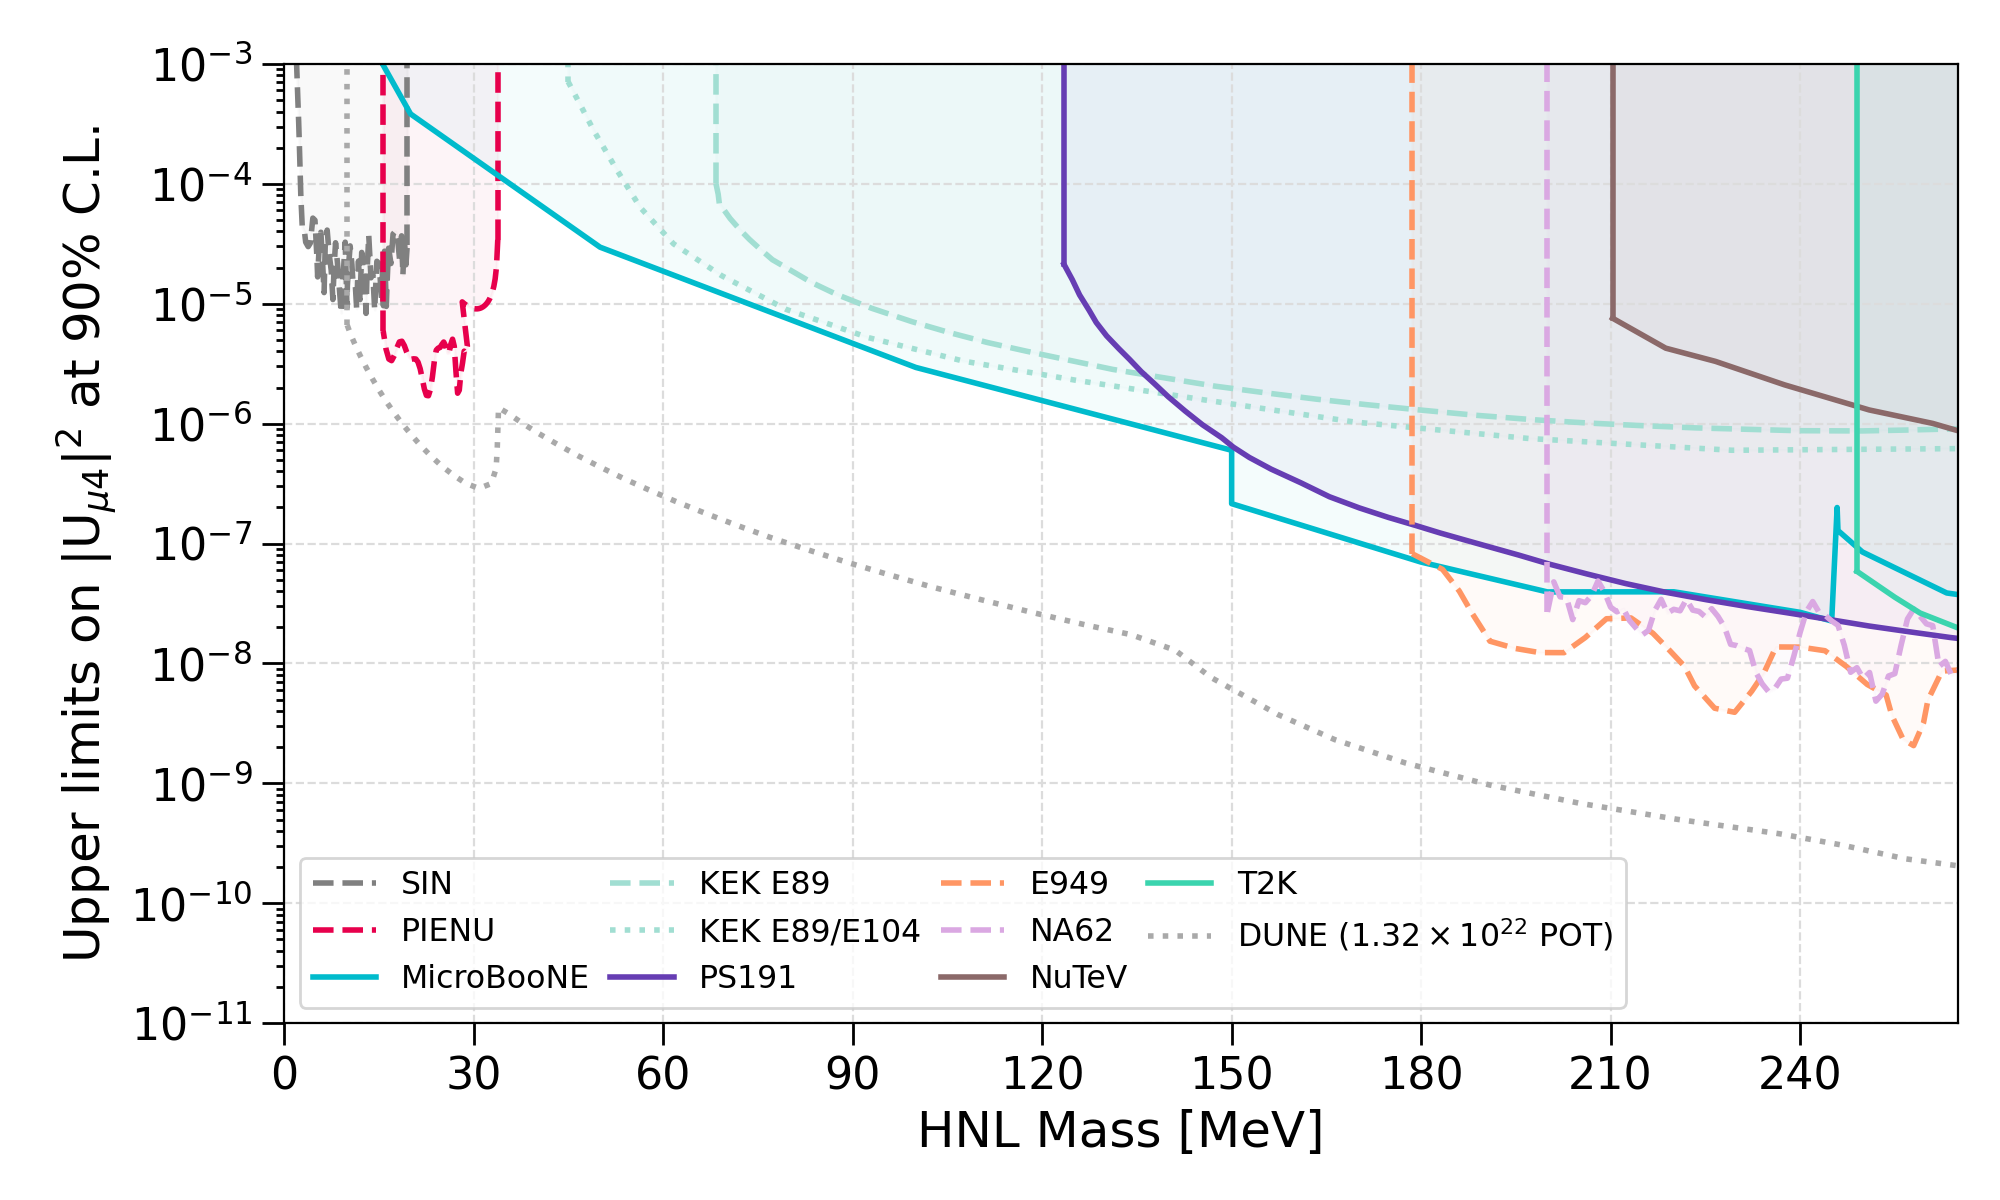
\includegraphics[width=1.0\textwidth]{sensitivity}
\caption[Sensitivity]{
Plot showing the upper limits on the mixing $|U_{\mu4}|^{2}$ at 90\% C.L. for Majorana HNLs in the mass range of $0 < m_{N} < 265$ MeV.
}
\label{fig:Sensitivity}
\end{figure}

\item The \textbf{MicroBooNE} collaboration conducted a series of searches for HNLs using their LArTPC, with the first result in 2020 and subsequent results in 2022 and 2023.
The initial analysis was performed using an exposure of $2 \times 10^{20}$ POT obtained from the on-axis BNB.
A special delayed trigger was implemented to identify HNLs arriving at the detector later than SM neutrinos.
Limits on $|U_{\mu4}|^{2}$ were set at $10^{-7}$ for HNL masses spanning between 260--385 MeV.
The latter two searches focused on HNLs arising from kaons decays in the NuMI beam absorber, which arrived at the detector at an angle to SM neutrinos from the BNB.
The dataset included two runs with an exposure of $2 \times 10^{20}$ and $5.01 \times 10^{20}$ POT.
The combined results incorporated multiple HNL decay channels, probing a wide mass spectrum between 10--385 MeV.
Notably, these recent results set the most stringent limits to date on $|U_{\mu4}|^{2}$ at 10$^{-4}$--10$^{-7}$ within the mass range of 34--175 MeV, extending the findings from 2019 \cite{uboone1, uboone2, uboone3}.

\end{coloritemize}

\section{Concluding Remarks}
\label{sec2conclude}

HNLs are beyond SM particles that can provide a natural explanation not just for the mass generation of active neutrinos but also for their extreme lightness.
SBND, located only 110 m from the BNB, is capable of detecting HNLs resulting from meson decays in the beam, which then decay in flight inside the detector.
Fig. \ref{fig:Sensitivity} provides a summary of existing limits on the mixing $|U_{\mu4}|^2$ of HNLs in the mass range of 0--265 MeV, showing that this phase space has been well-explored by various experiments very recently.
For SBND to be competitive in this region, a high background rejection rate without comprising signal efficiency must be achieved when performing the kinematic selection.
This can be obtained by exploiting kinematic observables of HNL decay products for background rejection, including their delay compared to SM neutrinos as well as their boosted kinematics due to HNLs being massive. 
Toward this goal, novel detection technology and reconstruction techniques of SBND have demonstrated an excellent resolution in timing, spatial and calorimetry. 
The following Chapter \ref{Chapter3} and \ref{ChapterDetector} will provide an overall description of the LArTPC technology, followed by details of the detection technology at SBND.
